\chapter{Methodology}
\label{chapt:methodology}


\section{Software}

\subsection{Nengo Package}

Summarize key constructs.

Resummarize Principle 3 with a focus on architecture / diagrams / Nengo code.

\subsection{NengoLib Package}

Summarize main contributions.
 - ZOH LIF
 - Multi-spiking LIF
 - RK45
 - Dynamic extensions
 - Geometric extensions
 - Temporal learning (offline), RLS (online alternative to PES)
 - FORCE, Reservoir Computing

\subsubsection{State-Space Realizations}

\subsubsection{Geometric Decoder Optimization}

\url{https://arvoelke.github.io/nengolib-docs/master/notebooks/research/geometric\_decoders.html}

\subsubsection{Encoders, Evaluation Points, and Semantic Pointers}

\subsubsection{Sampling High-Dimensional Vectors and Coordinates}

\subsubsection{Quanti-Monte Carlo Sampling}

\subsubsection{Leech Lattice}

Also mention?
Binary Semantic Pointers (generalized birthday paradox)
Locality Sensitive Hashing
See email chain on LSH. Also see email [cnrg-lab] bit of history

\subsubsection{Vector Oja Learning Rule}


\subsection{Hardware Backends}

nengo\_dl, nengo\_ocl, nengo\_fpga, nengo\_brainstorm, nengo\_loihi


\section{Optimization and Learning}

Some of this is going to be repetitive / overlapping with stuff from before, but I think they are the kind of things that are important to repeat...

We'll use this as an opportunity to point out the default scenario.

\subsection{Online versus Offline}

Online rules (PES, RLS), versus their offline analogs (stochastic gradient descent, least-squares)

\subsection{Explicit versus Implicit}

Using closed-form equations to generate the data (implicit), versus numerically simulating (explicit)

\subsection{Spikes versus Rates}

Learning from spikes versus learning from rates. And their equivalence in limiting conditions.

\section{Dynamics as a Language}

Everything can be specified at a high-level as a high-dimensional nonlinear dynamical system.

\subsection{Dynamics of Optimization Problems}

Mention nonlinear gradient-based algorithms 
 Compressed Sensing (LASSO / LCA)
 Expectation-Maximization
 PCA / SVD / ICA / NNMF

\subsection{Dynamics of WTA Circuits}

\subsection{Dynamics of Unsupervised Learning}

This section is taken from \citet{voelker2014a}. Also see \citet{trujillo2014a} and \citet{aubin2016a} and \citet{knight2016}.

Given a learning rate $\eta$, an input vector $x$ encoded by the activity of the input layer, the filtered activity $a(t)$ of  neurons in the middle layer, and the matrix $E$ whose rows are the ``preferred direction'' vectors of the middle layer neurons, we modify the preferred direction vectors of the middle layer neurons according to the equation:

\begin{align} \label{voja}
    \Delta{E} = \eta(a(t) x^T - a(t)E) = \eta a(t) (\begin{pmatrix}x^T \\ \vdots \\ x^T\end{pmatrix} - E)
\end{align}

Setting $\Delta{E_i} = 0$ gives $a_i(t)x = a_i(t)E_i$, and thus for a particular $x$, stability is characterized by

\begin{align} \label{stability}
    [\Delta{E_i} = 0]  \iff  [a_i(t) > 0  \implies  E_i = x]
\end{align}

Thus the effect of this rule is to make a subset of the middle layer neurons fire only when $x$ or a noisy version of it, is presented. The preferred direction vectors of the middle layer neurons are encoded in the synaptic weights between the first and middle layer neurons. Consequently, changing the preferred direction vectors corresponds to changing the connection weights using a local learning rule which we will outline in detail in the finished version.

\begin{figure}
    \centering
    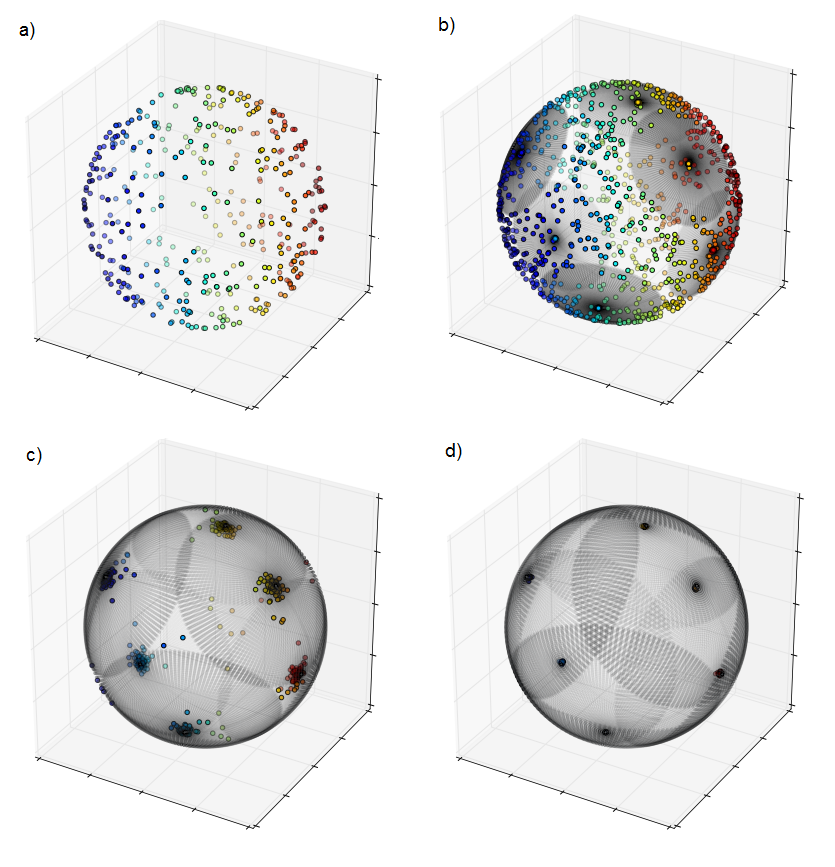
\includegraphics[width=0.8\textwidth]{voja-encoders}
    \caption{Input vector clustering of a 3-dimensional ensemble, presented with 6 evenly spaced $x$. (a) The initial clustering, before any input has been given. (b) Each input vector has been shown for 2 seconds of simulation time, with intercepts set to $cos(\frac{\pi}{6})$. Gray plates show the area of attraction for each input vector. (c) Same as b, with intercepts chosen to give $p_i = \frac{1}{6}$. (d) Same as b, with intercepts set to $cos(\frac{\pi}{3})$. \label{e3d}}
\end{figure}

\subsection{Dynamics of Supervised Learning}

This report is taken from \citep{voelker2015}.

Prescribed Error Sensitivity (PES) is a biologically plausible supervised learning rule that is frequently used with the Neural Engineering Framework (NEF). PES modifies the connection weights between populations of neurons to minimize an external error signal. We solve the discrete dynamical system for the case of constant inputs and no noise, to show that the decoding vectors given by the NEF have a simple closed-form expression in terms of the number of simulation timesteps. Moreover, with $\gamma = (1 - \kappa \|\V{a}\|^2) < 1$, where $\kappa$ is the learning rate and $\V{a}$ is the vector of firing rates, the error at timestep $k$ is the initial error times $\gamma^k$. Thus, $\gamma > - 1$ implies exponential convergence to a unique stable solution, $\gamma < 0 $ results in oscillatory weight changes, and $\gamma \le -1$ implies instability.

The Neural Engineering Framework (NEF), proposed by \citet{eliasmith2003a}, is a method of constructing biologically plausible spiking networks. To build and simulate such models, the Centre for Theoretical Neuroscience makes extensive use of the open-source software, Nengo \citep{bekolay2014}. 

The NEF typically learns its connection weights offline, but Nengo also supports a number of biologically plausible supervised and unsupervised learning rules to learn these weights online. By far, the most commonly used learning rule in Nengo is the Prescribed Error Sensitivity (PES) rule, which learns a function by minimizing an external error signal \citep{bekolay2013}. This learning rule has been used to model episodic memory \citep{trujillo2014}, hierarchical reinforcement learning \citep{rasmussen2014b}, adaptive motor control \citep{komer2015}, and many other tasks. 

While the usage and overall ``effect'' of the learning rule is intuitively clear, several questions have not been explicitly addressed to date:

\begin{itemize}
\item Under what conditions is the rule guaranteed to converge to a unique optimal solution?
\item How does the learning rate affect the rate of convergence?
\item Can we be precise about the form of the weights as a function of time, and the form of the optimal solution, if one exists?
\end{itemize}

This work aims to address all of these questions under the restricted setting of constant inputs and no noise.

\subsubsection{Prescribed Error Sensitivity}

For the analysis, we setup a network in Nengo containing an ensemble of $n$ neurons, inject a constant scalar input $x$, and minimize an error signal $e = y^* - y$ using the PES rule, where $y$ is the scalar output of the ensemble, and $y^*$ is the ideal output (see Fig.~\ref{fig:pes-dynamics-network}). The connection weights then learn to represent $y^*$ when presented with $x$. This work naturally extends to the case where $x$ is a vector, and so we only consider the scalar case for simplicity.

\begin{figure}
\centering
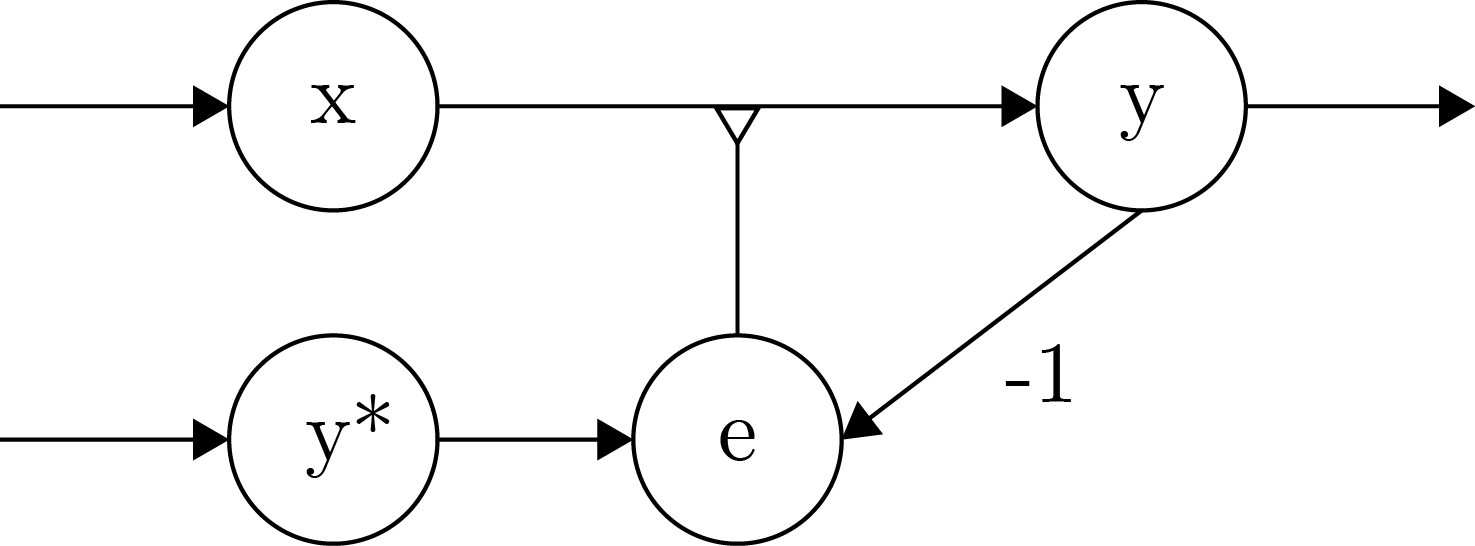
\includegraphics[width=0.6\textwidth]{pes-dynamics-network}
\caption{\label{fig:pes-dynamics-network} Network diagram used to analyze the PES rule. A connection from $x$ to $y$ learns to output $y^*$ by minimizing $|y^* - y|$. The error signal forms a modulatory connection to modify the weights between $x$ and $y$.}
\end{figure}

Let $\V{a} \in \mathbb{R}^n$ be the rate activity of each neuron without noise. This is given by the first principle of the NEF, and depends only on $x$. From here on we assume that $\V{a} \ne \V{0}$, otherwise our ensemble is not properly encoding $x$, in which case PES will have no effect. The PES rule then applies the following update rule at each timestep:
\begin{equation}
\label{eq:pes}
\Delta{\V{d}} = \kappa e \V{a}
\end{equation}
where $\kappa > 0$ is the learning rate, and $\V{d} \in \mathbb{R}^n$ is the decoding vector for the connection weight matrix such that, by the first principle of the NEF,
\begin{equation}
\label{eq:decoding}
y = \V{d}^T \V{a} .
\end{equation}

Now, to formulate the problem, let $\V{d}[k] \in \mathbb{R}^n$ be the value of the decoding vector $\V{d}$ at the $k^{th}$ timestep of the Nengo simulation, for all $k \in \mathbb{N}$. Our goal is to give a closed-form expression for $\V{d}[k]$ and its convergent solution. For notational convenience, the use of $\infty$ will imply a limit (e.g. $\V{d}[\infty] := \lim_{k \rightarrow \infty} \V{d}[k]$). Therefore, we will answer the following: given $\kappa$, $\V{a}$, $y^*$, and $\V{d}[0]$, what is $\V{d}[k]$ for $k \in \mathbb{N}$ and $\V{d}[\infty]$?

\begin{theorem}
\label{thm:pes-dynamics}

Let $\gamma = (1 - \kappa \|\V{a}\|^2) < 1$, and $e_0 = y^* - \V{d}[0]^T \V{a}$ be the initial error, then
\begin{align}
\label{eq:dk}
\V{d}[k] &= \V{d}[0] + e_0\frac{\V{a}}{\|\V{a}\|^2} (1 - \gamma^k)\text{, \quad $k \in \mathbb{N}$}
\end{align}
and so the error at timestep $k$ is $y^* - \V{d}[k]^T \V{a} = e_0\gamma^k$. In particular, if $\gamma > - 1$, then $\V{d}[\infty]$ exists and is given by the unique solution,
\begin{align}
\label{eq:dinf}
\V{d}[\infty] &= \V{d}[0] + e_0\frac{\V{a}}{\|\V{a}\|^2} .
\end{align}

On the other hand, if $\gamma \le -1$ then the system is unstable.
\end{theorem}

\paragraph{Discussion}

An immediate consequence is that the error $y^* - y$ goes to 0 exponentially with rate $\gamma$. When $\gamma < 0$, this results in oscillations around the optimal solution. When $\gamma > - 1$, the limit exists and is given by the stable optimum (\ref{eq:dinf}). 

The error given by (\ref{eq:dk}) implies that if we desire an approximation factor of $\epsilon$ times the initial error in $k$ timesteps, then set the learning rate to $$\kappa = (1 - \epsilon^{1/k}) / \|a\|^2.$$

The theorem essentially states that the optimal solution is achieved by increasing the decoders by the normalized activity vector scaled by the initial error. In hindsight, this should be somewhat intuitive. If we look at (\ref{eq:pes}), only a scaled version of $\V{a}$ is ever added to the decoders, and so it makes sense that the final difference could only be some multiple of $\V{a}$. If we suppose that $\V{d}[\infty]$ converges, and furthermore $\V{d}[\infty]^T \V{a} = y^*$, then we may indeed solve $\V{d}[\infty]^T \V{a} = \V{d}[0]^T \V{a} + \alpha \V{a}^T \V{a}$ for the required scaling factor $\alpha = \frac{e_0}{\V{a}^T \V{a}}$. Conversely, we can verify that indeed the above $\V{d}[\infty]$ decodes $y^*$ by evaluating $\V{d}[\infty]^T \V{a} = \V{d}[0]^T \V{a} + e_0 \frac{\V{a}^T\V{a}}{\V{a}^T\V{a}} = y^*$.

However, this is not a proof, since we have supposed that the optimal solution exists and is unique, while there are infinitely many solutions to $\V{u}^T \V{a} = y^*$. Specifically, $\V{u} = \V{d}[\infty] + \V{v}$, where $\V{v}^T \V{a} = 0$, all of which are stable since they have zero error. We must therefore show that only one of these solutions is reachable (namely $\V{v} = \V{0}$), and that $\gamma$ gives the exponential rate of convergence.

\paragraph{Proof of Theorem~\ref{thm:pes-dynamics}}

The first step is to formulate the equation for $\V{d}[k]$ using linear algebra. Let $k \in \mathbb{N}$. Combining (\ref{eq:pes}) and (\ref{eq:decoding}) with $e = y^* - y$, gives us:
\begin{align*}
\V{d}[k+1]^T &= \V{d}[k]^T + \kappa(y^* - \V{d}[k]^T \V{a})\V{a}^T \\ 
         &= \V{d}[k]^T\underbrace{(I - \kappa \V{a}\V{a}^T)}_{A} + \underbrace{\kappa y^* \V{a}^T}_{\V{c}^T} .
\end{align*}

The last two components are labeled by the matrix $A \in \mathbb{R}^{n,n}$ and the vector $\V{c} \in \mathbb{R}^{n}$, since they will appear frequently throughout the analysis. This also allows us to express the above relationship compactly as:
\begin{equation}
\label{eq:statespace}
\V{d}[k+1]^T = \V{d}[k]^T A + \V{c}^T.
\end{equation}

It is important to note that neither $A$ nor $\V{c}$ depend on $\V{d}[k]$. $A$ depends solely on $\V{a}$, which is fixed for a given $x$ by the first principle of the NEF. $\V{c}$ depends only on $\V{a}$ and $y^*$, which are again also fixed. Therefore, $\V{d}[k]$, and thus $\V{d}[\infty]$, can be found inductively:
\begin{equation}
\label{eq:dksum}
\V{d}[k]^T = \V{d}[0]^T A^k + \sum_{i=0}^{k-1} \V{c}^T A^i.
\end{equation}

In order to find a closed-form expression for (\ref{eq:dksum}) we must essentially characterize the effect of repeated multiplication and addition by using the eigendecomposition of the system. This is done by interpreting (\ref{eq:statespace}) as the {\it state-space representation} of a discrete linear control system with constant input, where the ``state'' is given by the current decoders. Since $A$ is symmetric, this is also equivalent to $\V{d}[k+1] = A \V{d}[k] + \V{c}$, but it turns out that the eigendecomposition of the former system has a nicer interpretation.

We proceed with some basic results on $A = I - \kappa \V{a}\V{a}^T$, and then move toward a construction that reveals the eigenvectors of the whole system, which in turn proves the main theorem.

Since $A$ is symmetric, by the spectral theorem it can be diagonalized to $A = VWV^T$, where $V$ is orthonormal ($V^{-1} = V^T$), and $W$ is diagonal. Moreover, the columns of $V$ are the unit eigenvectors of $A$ (giving us an $n$-dimensional eigenbasis), and their corresponding eigenvalues are on the respective diagonals in $W$. Now, since $A$ differs only from $I$ by an outer product, it has very specific structure.

\begin{lemma}\label{lemma:1} $\V{a}$ is an eigenvector of $A$ with eigenvalue $\gamma < 1$.\end{lemma}

\begin{proof} Recalling that $\gamma = 1 - \kappa \|\V{a}\|^2$,
\begin{align*}
A\V{a} &= (I - \kappa \V{a}\V{a}^T)\V{a} \\
   &= (\V{a} - \V{a} \kappa \V{a}^T\V{a}) \\
   &= \gamma \V{a}
\end{align*}

Since $\V{a} \ne 0$ is non-negative, we know $\|\V{a}\|^2 > 0$ (and $\kappa > 0$), thus $\gamma < 1$.
\end{proof}

\begin{lemma}\label{lemma:2} The remaining $n-1$ eigenvectors of $A$ are orthogonal to $\V{a}$ with eigenvalue 1.\end{lemma}

\begin{proof} The first part follows trivially from the fact that $A$ can be diagonalized and so the remaining $n-1$ dimensions must span a subspace that is orthogonal to $\V{a}$ (by lemma \ref{lemma:1}). To be precise, the remaining eigenvectors form an orthonormal basis for the nullspace of $\V{a}^T$, with eigenvalue 1, because
$A\V{u} = \V{u} \IFF ( I - \V{a}\V{a}^T ) \V{u} = \V{u} \IFF \V{0} = \V{a}\V{a}^T\V{u} \IFF \V{a}^T \V{u} = 0$, since $\V{a} \ne 0$.
\end{proof}

Geometrically, this means that the mapping $A$ modifies a single dimension of the vector, namely the line spanning $\V{a}$ with eigenvalue $\gamma < 1$. The remaining portion, in the hyperplane orthogonal to $\V{a}$, remains untouched. Given conditions on $\kappa$ so that $\gamma > -1$, in the limit $A^\infty$ will zero out the dimension spanned by $\V{a}$. In fact, these two lemmas are enough to diagonalize $A$, which we use to show that $A^\infty = I - \frac{\V{a}\V{a}^T}{\|\V{a}\|^2}$ (below). This makes intuitive sense since $P_\V{a} = \frac{\V{a}\V{a}^T}{\|\V{a}\|^2}$ is a projection onto $\V{a}$, and so $A^\infty \V{u} = \V{u} - P_\V{a} \V{u}$ gives us the portion of $\V{u}$ that is orthogonal to $\V{a}$. To see this more rigorously, let $V_0$ be equal to $V$ with all but its first column ($\frac{\V{a}}{\|\V{a}\|}$) set to zero. That is, $V = V_0 + \begin{pmatrix}0 & V_1\end{pmatrix}$. Then since the first diagonal of $W^\infty$ goes to zero,
\begin{align*}
A^\infty &= VW^\infty V^T \\
         &= (V - V_0)V^T \\
         % (&= V_1 V^T = V_1 V_1^T) \\
         &= I - V_0 V^T \\
         &= I - \frac{\V{a}}{\|\V{a}\|}\frac{\V{a}^T}{\|\V{a}\|} \\
         &= I - \frac{\V{a}\V{a}^T}{\|\V{a}\|^2} .
\end{align*}

Of course, this is only half the story, since we have not yet involved $\V{c}$, which is the sole bearer of $y^*$. To this end, we use the following construction:
\begin{equation*}
\tilde{A} = \begin{pmatrix}
A & \V{0} \\
\V{c}^T & 1
\end{pmatrix} \in \mathbb{R}^{n+1,n+1}, \quad \V{\tilde{d}}[k] = \begin{pmatrix}\V{d}[k] \\ 1\end{pmatrix} \in \mathbb{R}^{n+1}.
\end{equation*}
It is easy to see that $\V{\tilde{d}}[k]^T \tilde{A}$ will multiply $\V{d}[k]^T$ by $A$ and add $\V{c}^T$, so by induction this allows us to rewrite (\ref{eq:statespace}) as a single matrix multiply:
\begin{equation}
\label{eq:system}
\V{\tilde{d}}[k]^T = \V{\tilde{d}}[0]^T \tilde{A}^k .
\end{equation}

%We now show that $\tilde{A}$ can be diagonalized using the eigendecomposition of $A$.

\begin{lemma}\label{lemma:3} Let $\beta = \frac{\V{c}^T \V{a}}{(\gamma - 1)\|\V{a}\|}$, then $\V{\tilde{a}} = \begin{pmatrix}\frac{\V{a}}{\|\V{a}\|} \\ \beta \end{pmatrix}$ is an eigenvector of $\tilde{A}$ with eigenvalue $\gamma$.\end{lemma}

\begin{proof}$\V{\tilde{a}}$ is well-defined since $\gamma < 1$.
 
$\tilde{A}\V{\tilde{a}} = \begin{pmatrix}\frac{A\V{a}}{\|\V{a}\|} \\ \V{c}^T\frac{\V{a}}{\|\V{a}\|} + \beta\end{pmatrix} = \begin{pmatrix}\frac{\gamma \V{a}}{\|\V{a}\|} \\ \frac{\V{c}^T \V{a} \gamma}{(\gamma - 1)\|\V{a}\|}\end{pmatrix} = \gamma \V{\tilde{a}}$, by lemma \ref{lemma:1}.\end{proof}

We remark that the last component of $\V{\tilde{a}}$ can be simplified to: $$\beta = \frac{\V{c}^T \V{a}}{(\gamma - 1)\|\V{a}\|} = \frac{\kappa y^* \V{a}^T \V{a}}{- \kappa \|\V{a}\|^2 \|\V{a}\|} = -\frac{y^*}{\|\V{a}\|}.$$

\begin{lemma}\label{lemma:4} Suppose $\V{u}$ is an eigenvector of $A$ such that $A\V{u} = \V{u}$, then $\V{\tilde{u}} = \begin{pmatrix}\V{u} \\ 0\end{pmatrix}$ similarly satisfies $\tilde{A}\V{\tilde{u}} = \V{\tilde{u}}$.\end{lemma}

\begin{proof}$$\tilde{A}\V{\tilde{u}} = \begin{pmatrix}A\V{u} \\ \V{c}^T \V{u} \end{pmatrix} = \begin{pmatrix}\V{u} \\ \kappa y^* \V{a}^T \V{u} \end{pmatrix} = \begin{pmatrix}\V{u} \\ 0 \end{pmatrix} = \V{\tilde{u}}$$ since $\V{a}^T \V{u} = 0$ from lemma \ref{lemma:2}.\end{proof}

Now observe that $(0, 0, \ldots, 1)^T \in \mathbb{R}^{n+1}$ is an eigenvector for $\tilde{A}$ with eigenvalue 1, and so we have found $n+1$ eigenvectors for $\tilde{A}$. Recall that $A = VWV^T$. Without loss of generality, suppose the columns of $V$ are arranged so that $\frac{\V{a}}{\|\V{a}\|}$ is the first column (using lemma \ref{lemma:1}). Then, construct $\V{b} = (\beta, 0, \ldots, 0)^T \in \mathbb{R}^{n+1}$, and place all $n+1$ eigenvectors in a square matrix,
$$\tilde{V} = \begin{pmatrix} V & \V{0} \\ \V{b}^T & 1\end{pmatrix}$$
with corresponding eigenvalues
$$\tilde{W} = \begin{pmatrix} W & \V{0} \\ \V{0}^T & 1\end{pmatrix}.$$

Then $\tilde{A}\tilde{V} = \tilde{V}\tilde{W}$ by lemmas \ref{lemma:3} and \ref{lemma:4}. To complete the diagonalization, we must show that $\tilde{V}$ is invertible by arguing that the eigenvectors we found are linearly independent, or better yet by explicitly constructing the inverse:
$$\tilde{V}^{-1} = \begin{pmatrix}V^T & \V{0} \\- \V{b}^T V^T & 1\end{pmatrix} = \begin{pmatrix}V^T & \V{0} \\ - \beta \frac{\V{a}^T}{\|\V{a}\|} & 1\end{pmatrix}.$$ 

Finally, we are ready to diagonalize $\tilde{A}$:
\begin{lemma}\label{lemma:5} $\tilde{A} = \tilde{V}\tilde{W}\tilde{V}^{-1} = \begin{pmatrix} V & \V{0} \\ \V{b}^T & 1\end{pmatrix} \begin{pmatrix} W & \V{0} \\ \V{0}^T & 1\end{pmatrix} \begin{pmatrix}V^T & \V{0} \\- \V{b}^T V^T & 1\end{pmatrix}$.\end{lemma}

\begin{proof}$$\tilde{V}\tilde{V}^{-1} = \begin{pmatrix} 
V & \V{0} \\ 
\V{b}^T & 1\end{pmatrix} \begin{pmatrix}
V^T & \V{0} \\
- \V{b}^T V^T & 1\end{pmatrix} = \begin{pmatrix}
VV^T & \V{0} \\
\V{b}^TV^T - \V{b}^T V^T & 1\end{pmatrix} = I$$\end{proof}

We are now ready to prove the main theorem. The purpose of obtaining the above diagonalization is that it enables us to give a closed-form solution for $\V{\tilde{d}}[k]$ via (\ref{eq:system}) and lemma \ref{lemma:5}. Let $V_1 \in \mathbb{R}^{n,n-1}$ be equal to $V$ without its first column, such that $V = \begin{pmatrix}\frac{\V{a}}{\|\V{a}\|} & V_1\end{pmatrix}$.
\begin{align*}
\label{eq:diag}
\V{d}[k]^T &= \begin{pmatrix}\V{d}[0] \\ 1\end{pmatrix}^T \begin{pmatrix} \frac{\V{a}}{\|\V{a}\|} & V_1 & 0 \\ \beta & \V{0}^T & 1\end{pmatrix} \begin{pmatrix} \gamma^k & & & \\ & 1 & & \\ & & \ddots & \\ & & & 1 \end{pmatrix} \begin{pmatrix}\frac{\V{a}^T}{\|\V{a}\|} \\ V_1^T \\- \beta \frac{\V{a}^T}{\|\V{a}\|} \end{pmatrix} \\
       &= \begin{pmatrix}\V{d}[0]^T\frac{\V{a}}{\|\V{a}\|} + \beta & \V{d}[0]^T V_1 & 1\end{pmatrix} \begin{pmatrix} \gamma^k & & & \\ & 1 & & \\ & & \ddots & \\ & & & 1 \end{pmatrix} \begin{pmatrix}\frac{\V{a}^T}{\|\V{a}\|} \\ V_1^T \\- \beta \frac{\V{a}^T}{\|\V{a}\|} \end{pmatrix} \\
       &= \begin{pmatrix}\gamma^k(\V{d}[0]^T\frac{\V{a}}{\|\V{a}\|} + \beta) & \V{d}[0]^T V_1 & 1\end{pmatrix} \begin{pmatrix}\frac{\V{a}^T}{\|\V{a}\|} \\ V_1^T \\- \beta \frac{\V{a}^T}{\|\V{a}\|} \end{pmatrix} \\
       &= \gamma^k(\V{d}[0]^T\frac{\V{a}}{\|\V{a}\|} + \beta) \frac{\V{a}^T}{\|\V{a}\|} + \V{d}[0]^T V_1 V_1^T - \beta \frac{\V{a}^T}{\|\V{a}\|} \\
       &= \V{d}[0]^T (I - \frac{\V{a}\V{a}^T}{\|\V{a}\|^2}) + \frac{y^*}{\|\V{a}\|^2} \V{a}^T - \gamma^k(y^* - \V{d}[0]^T \V{a}) \frac{\V{a}^T}{\|\V{a}\|^2} \\
       &= \V{d}[0]^T + e_0 \frac{\V{a}^T}{\|\V{a}\|^2} (1 - \gamma^k)       
\end{align*}

To find the limit as $k \rightarrow \infty$, recall from lemmas \ref{lemma:3} and \ref{lemma:4} that the spectrum of the system is $sp(\tilde{A}) = sp(A) = \{\gamma, 1, 1, ...\}$, by lemma \ref{lemma:1}. Thus, (\ref{eq:system}) requires that $|\gamma| < 1$ in order for $\V{d}[\infty]$ to exist. Since $\gamma < 1$, $\V{d}[\infty]$ converges $\IFF \gamma > -1$. If $\gamma \le -1$, then the state explodes. In the stable condition,
\begin{equation*}
\V{d}[\infty]^T = \V{d}[0]^T\underbrace{(I - \frac{\V{a}\V{a}^T}{\|\V{a}\|^2})}_{A^\infty} + \underbrace{\frac{y^*}{\|\V{a}\|^2} \V{a}^T}_{\sum_{i=0}^{\infty} \V{c}^T A^i}
\end{equation*}

To get the error at timestep $k$, we use (\ref{eq:decoding}) to obtain
\begin{equation*}(\V{d}[\infty]^T - \V{d}[k]^T)\V{a} = e_0 \gamma^k \frac{\V{a}^T \V{a}}{\|\V{a}\|^2} = e_0 \gamma^k\end{equation*}
which concludes the proof. \hfill $\square$

\begin{figure}
\centering
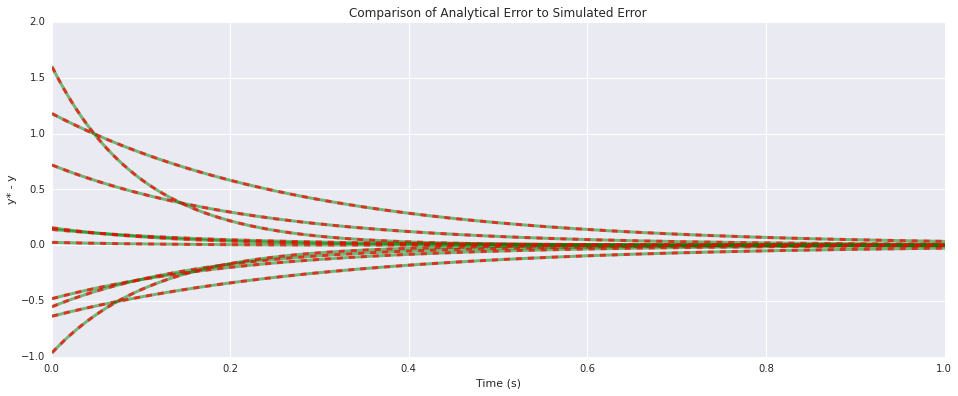
\includegraphics[width=1.0\textwidth]{pes-dynamics-validation}
\caption{\label{fig:pes-dynamics-validation} Comparison of the analytical error given by the theorem to the simulated error in Nengo. Each line indicates the error $y^* - y$ over time for a single trial, for a random number of rate neurons (noiseless) from the range $
[10, 200]$, a random learning rate from $[10^{-6}, 5 \times 10^{-4}]$, a random $x$ from $[-1, 1]$, and a random $y^*$ from $[-1, 1]$. In all trials, the analytical error is shown with a dashed line, with a root-mean-square error of less than $10^{-14}$.}
\end{figure}

This report is taken from \citep{voelker2017c}.

Prescribed Error Sensitivity (PES) is a biologically plausible supervised learning rule that is frequently used with the Neural Engineering Framework (NEF).
PES modifies the connection weights between populations of spiking neurons to minimize an error signal.
Continuing the work of Voelker (2015), we solve for the dynamics of PES, while filtering the error with an arbitrary linear synapse model. 
For the most common case of a lowpass filter, the continuous-time weight changes are characterized by a second-order bandpass filter with frequency $\omega = \sqrt{\tau^{-1} \kappa \|\V{a}\|^2 }$ and bandwidth $Q = \sqrt{\tau \kappa \|\V{a}\|^2 }$, where $\tau$ is the exponential time constant, $\kappa$ is the learning rate, and $\V{a}$ is the activity vector.
Therefore, the error converges to zero, yet oscillates if and only if $\tau \kappa \|\V{a}\|^2 > \frac{1}{4}$.
This provides a heuristic for setting $\kappa$ based on the synaptic $\tau$, and a method for engineering remarkably accurate decaying oscillators using only a single spiking leaky integrate-and-fire neuron.

The Neural Engineering Framework~\citep[NEF;][]{eliasmith2003a} is a method for constructing biologically plausible spiking networks.
To build and simulate such models, the Centre for Theoretical Neuroscience makes extensive use of the open-source software, Nengo~\citep{bekolay2014}. 
Nengo typically learns its connection weights offline, but also supports a number of biologically plausible supervised and unsupervised learning rules to learn its weights online.
By far, the most commonly used learning rule in Nengo is the Prescribed Error Sensitivity~\citep[PES;][]{bekolay2013} rule, which learns a function by minimizing a supervised error signal from external and recurrent feedback.

Previously, \citet{voelker2015} fully characterized the discrete-time dynamics of PES under the restricted setting of a constant input signal, constant reference signal, and no noise.
Due to the absence of noise, no filter was required for the error signal.
However, for spiking networks considered in practice, a lowpass is applied to the error to filter out spike-noise~\citep[e.g.,][]{dewolf2016, rasmussen2017},  

In this report, we relax the assumption of a constant reference signal, and apply an arbitrary linear filter to the error signal.
For simplicity, we do so for the case of a continuous-time simulation, but our analysis can also be applied to the discrete-time setting via the $Z$-transform.
To keep our analysis tractable, we still assume a constant input signal, and briefly discuss implications for the general dynamic setting.

We begin by formulating a mathematical description of the network, present our theoretical results, prove them mathematically, validate them with numerical simulations, and demonstrate the utility of this analysis by engineering oscillators with predetermined frequencies and decay rates.
Finally, we conclude by discussing some implications of this report for learning spiking dynamical networks online.

\subsubsection{Prescribed Error Sensitivity}

\begin{figure}
\centering
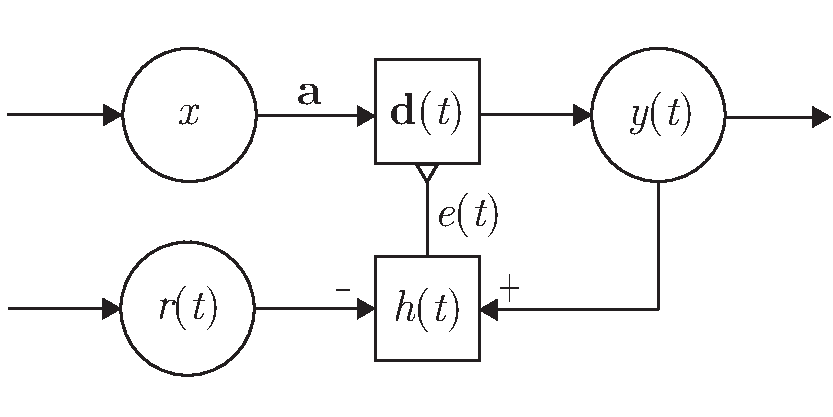
\includegraphics[width=0.8\textwidth]{pes-filtered-network}
\caption{\label{fig:pes-filtered-network}
  Network diagram used to analyze the PES rule.
  A constant input $x$ is represented by a population of $n$ spiking neurons with the activity vector $\V{a} \in \mathbb{R}^n$.
  A dynamic reference signal $r(t)$ determines the error $e(t) = \left((y - r) \ast h\right)(t)$~(equation~\ref{eq:error}), which in turn drives $y(t)$ towards $r(t)$ by modulating the connection weights via PES~(equation~\ref{eq:pes}).
  These learned connection weights decode $y(t)$ via the decoders $\V{d}(t) \in \mathbb{R}^n$~(equation~\ref{eq:decoding}).
  A linear filter $h(t)$ models the postsynaptic current induced by each spike.
}
\end{figure}

Consider a network in Nengo, containing a population of $n$ spiking neurons, encoding the constant scalar input $x$.
Let $\V{a} \in \mathbb{R}^n$ be the average (i.e.,~rate) activity of each neuron in response to this encoding.\footnote{Here on, we assume that $\V{a} \ne \V{0}$, otherwise PES will have no effect.}
This vector is determined by the first principle of the NEF, and remains fixed for constant $x$.
The \emph{decoders} $\V{d}(t) \in \mathbb{R}^n$ determine the scalar output $y(t)$ via the dot-product:
\begin{equation}
\label{eq:decoding}
y(t) = \transpose{\V{a}} \V{d}(t)  \text{.}
\end{equation}
The PES rule learns these decoders, online, according to the following dynamics:
\begin{equation}
\label{eq:pes}
\dot{\V{d}}(t) = -\kappa e(t) \V{a} \text{,}
\end{equation}
where $\kappa > 0$ is the learning rate,\footnote{$\kappa$ is automatically scaled by $n^{-1}$ in Nengo, to balance the linear scaling of $\|\V{a}\|^2$.} and $e(t)$ is the chosen error signal:\footnote{Signs are flipped in \citet{voelker2015}; equations~\ref{eq:pes} and~\ref{eq:error} are consistent with Nengo.}
\begin{equation}
\label{eq:error}
e(t) = \left((y - r) \ast h \right)(t) \text{,}
\end{equation}
where $r(t)$ is the reference (i.e.,~ideal) output, and $h(t)$ is some arbitrary linear filter modeling the postsynaptic current (PSC) induced by a spike arriving at the synaptic cleft.
Typically, $h(t)$ is a first-order lowpass filter with time constant~$\tau > 0$ (i.e.,~modeling an exponentially decaying PSC): %, sometimes also referred to as a ``leaky integrator'':
\begin{equation}
\label{eq:lowpass}
h(t) = \frac{1}{\tau} e^{-\frac{t}{\tau}} \iff H(s) = \frac{1}{\tau s + 1} \text{.\footnotemark}
\end{equation}
\footnotetext{Capital-case variables denote the Laplace transforms of their corresponding lower-case (time-domain) variables.}%
%Thus, the connection weights learn to represent $r$ when presented with $x$.
The final network is summarized in Figure~\ref{fig:pes-filtered-network}.
This also naturally extends to the case where $x$ and $y$ are vectors (using a population code), but we consider the scalar case for simplicity. 

Now, we aim to characterize the dynamics of $e(t)$ in response to the control signal $r(t)$.
Alternatively, we could characterize the dynamics of $y(t)$ or $\V{d}(t)$, but the former is easier to work with, while describing the latter via equations~\ref{eq:decoding} and~\ref{eq:pes} (i.e.,~by integrating $e(t)$).

\begin{theorem}
\label{thm:pes-filtered}
Let $\phi = \tau \kappa \|\V{a}\|^2$.
For the network described in Figure~\ref{fig:pes-filtered-network}, we have:
\begin{equation}
\label{eq:time-domain}
e(t) = (r \ast f)(t) \text{,}
\end{equation}
where: %\footnote{$\mathcal{L}^{-1} \left\{ \cdot \right\}$ denotes the inverse Laplace transform.}
\begin{equation}
\label{eq:s-domain}
F(s) = \frac{-s}{s H(s)^{-1} + \kappa \|\V{a}\|^2} \text{,} 
%f(t) &= \mathcal{L}^{-1} \left\{ F(s) \right\} \\
%H(s) &= \mathcal{L} \left\{ H(t) \right\} \text{.}
\end{equation}
hence $F(s)$ is the transfer function from $R(s)$ to $E(s)$.
For the case of a first-order lowpass filter (equation~\ref{eq:lowpass}),
\begin{align}
\label{eq:lowpass-solution}
\implies \quad F(s) = \frac{-s}{\tau s^2 + s + \kappa \|\V{a}\|^2} &= \frac{-\left( \kappa \|\V{a}\|^2 \right)^{-1} s}{\left(\frac{1}{\omega^2}\right)s^2 + \left(\frac{1}{\omega Q}\right) s + 1} \quad\quad \\
\omega &= \sqrt{\tau^{-1} \kappa \|\V{a}\|^2 } \label{eq:bandpass-w} = \tau^{-1} \sqrt{\phi} \\
Q &= \sqrt{\tau \kappa \|\V{a}\|^2 } = \sqrt{\phi} \label{eq:bandpass-Q} \text{.}
\end{align}
Thus, $F(s)$ is a second-order $Q$-bandpass filter with frequency $\omega$ in radians per second ($\frac{\omega}{2 \pi}$ is the frequency in hertz)~\citep[][pp.~8.9--8.10]{zumbahlen2011linear}.
The poles of $F(s)$ are:
\begin{equation}
\label{eq:poles}
s = \frac{-1 \pm \sqrt{1 - 4 \phi}}{2\tau} \text{.}
\end{equation}
%with complex magnitude $|s| = \omega$.
Since $\phi > 0$, this system is exponentially stable, and, moreover, the impulse response, $f(t)$, is a decaying oscillator if and only if $\phi > \frac{1}{4}$.
\end{theorem}

\begin{proof}
We begin by transforming equations~\ref{eq:decoding}--\ref{eq:error} into the Laplace domain:
\begin{align*}
Y(s) &= \transpose{\V{a}} \V{D}(s) \\
s\V{D}(s) &= - \kappa E(s) \V{a} \\
E(s) &= \left(Y(s) - R(s) \right) H(s) \text{.\footnotemark}
\end{align*}
\footnotetext{This has nice form since $\V{a}$ is a constant -- otherwise multiplication of two time-varying signals becomes a complex integral in the Laplace domain.}%
Substituting the first two equations into the last, yields:
\begin{align*}
&& E(s) &= \left( \transpose{\V{a}} \V{D}(s) - R(s) \right) H(s) \\
&& &= \left( - \transpose{\V{a}} s^{-1} \kappa E(s) \V{a} - R(s) \right) H(s) \\
&& &= - \kappa \|\V{a}\|^2 s^{-1} H(s) E(s) - R(s) H(s) \\
\iff && \left(1 + \kappa \|\V{a}\|^2 s^{-1} H(s) \right) E(s) &= - R(s) H(s) \\
\iff && E(s) &= R(s) \left( \frac{-H(s)}{1 + \kappa \|\V{a}\|^2 s^{-1} H(s)} \right) \\
&& &= R(s) \left( \frac{- s}{s H(s)^{-1} + \kappa \|\V{a}\|^2} \right) \\
&& &= R(s) F(s) \text{.} \tag*{\qed}
\end{align*}

Equations~\ref{eq:time-domain} and~\ref{eq:s-domain} follow from the convolution theorem.
Equations~\ref{eq:lowpass-solution}--\ref{eq:bandpass-Q} are verified by substituting $H(s)^{-1} = \tau s + 1$ into equation~\ref{eq:s-domain}.

The poles of the system (equation~\ref{eq:poles}) are obtained by applying the quadratic formula to the denominator polynomial from equation~\ref{eq:lowpass-solution} ($\tau s^2 + s + \kappa \|\V{a}\|^2$).
%The magnitude of the poles ($\omega$) come from the polar coordinate solution to this quadratic.
Exponential stability is implied by both poles being strictly in the left half-plane.
Lastly, $f(t)$ oscillates if and only if the poles are complex, if and only if the discriminant ($1 - 4 \phi$) is negative, if and only if $\phi > \frac{1}{4}$.
\end{proof}

%As a corollary to equation~\ref{eq:lowpass-solution} and the Laplace transform of equations~\ref{eq:decoding} and~\ref{eq:pes},
%\begin{equation}
%y(t) = (r \ast g)(t) \text{,}
%\end{equation}
%where:
%\begin{equation}
%G(s) = \frac{\kappa \|a\|^2}{\tau s^2 + s + %\kappa \|\V{a}\|^2} \text{,}
%\end{equation}
%which has the same dynamics as equation~\ref{eq:lowpass-solution} with a phase shift.
%But these are (unfiltered) spikes...

\subsubsection{Validation}

We construct the network from Figure~\ref{fig:pes-filtered-network} using Nengo~2.5.0~\citep{bekolay2013}, $n = 1$ spiking leaky integrate-and-fire neurons (mean firing rate of $262\,$Hz),\footnote{Spikes are used in place of $\V{a}$ in equations~\ref{eq:decoding} and~\ref{eq:pes}.} $\tau = 0.1\,$s (equation~\ref{eq:lowpass}), $x = 0$, and $\kappa$ such that $\phi > \frac{1}{4}$.
We construct the transfer function from equation~\ref{eq:lowpass-solution} using nengolib~0.4.0~\citep{nengolib}:
\begin{python}
import nengolib
from nengolib.signal import s
H = nengolib.Lowpass(tau)
F = -s / (s/H + kappa*a.dot(a))
\end{python}
where \texttt{tau}~$\leftarrow \tau$ is the time constant of the synapse, \texttt{kappa}~$\leftarrow \kappa$ is the learning-rate supplied to Nengo (divided by $n$), and \texttt{a}~$\leftarrow \V{a}$ is the NumPy array for the population's activity.
We evaluate $(r \ast f)(t)$ using \texttt{F.filt(r, dt=dt)}, and compare this to the $e(t)$ obtained numerically in simulation.
The \texttt{filt} method automatically discretizes $F(s)$ according to the simulation time-step (\texttt{dt}~$= 1\,$ms) using zero-order hold (ZOH).\footnote{Technically, for a discrete-time simulation, the problem and results should have been formulated in the discrete-time domain using the $Z$-transform to begin with, as opposed to discretizing at the end, but the difference is quite subtle.}

In Figure~\ref{fig:pes-error}, we confirm that $(r \ast f)(t)$ approximates the numerical $e(t)$ given white noise $r(t)$.
In Figure~\ref{fig:pes-oscillator}-Top, we exploit our knowledge of the impulse response, $f(t)$, to engineer a number of decaying oscillators by controlling $r(t)$.
In Figure~\ref{fig:pes-oscillator}-Bottom, we evaluate \texttt{np.abs(F.evaluate(freqs))} at a variety of frequencies (\texttt{freqs}) to visualize the bandpass behaviour of each filter.

\begin{figure}
\centering
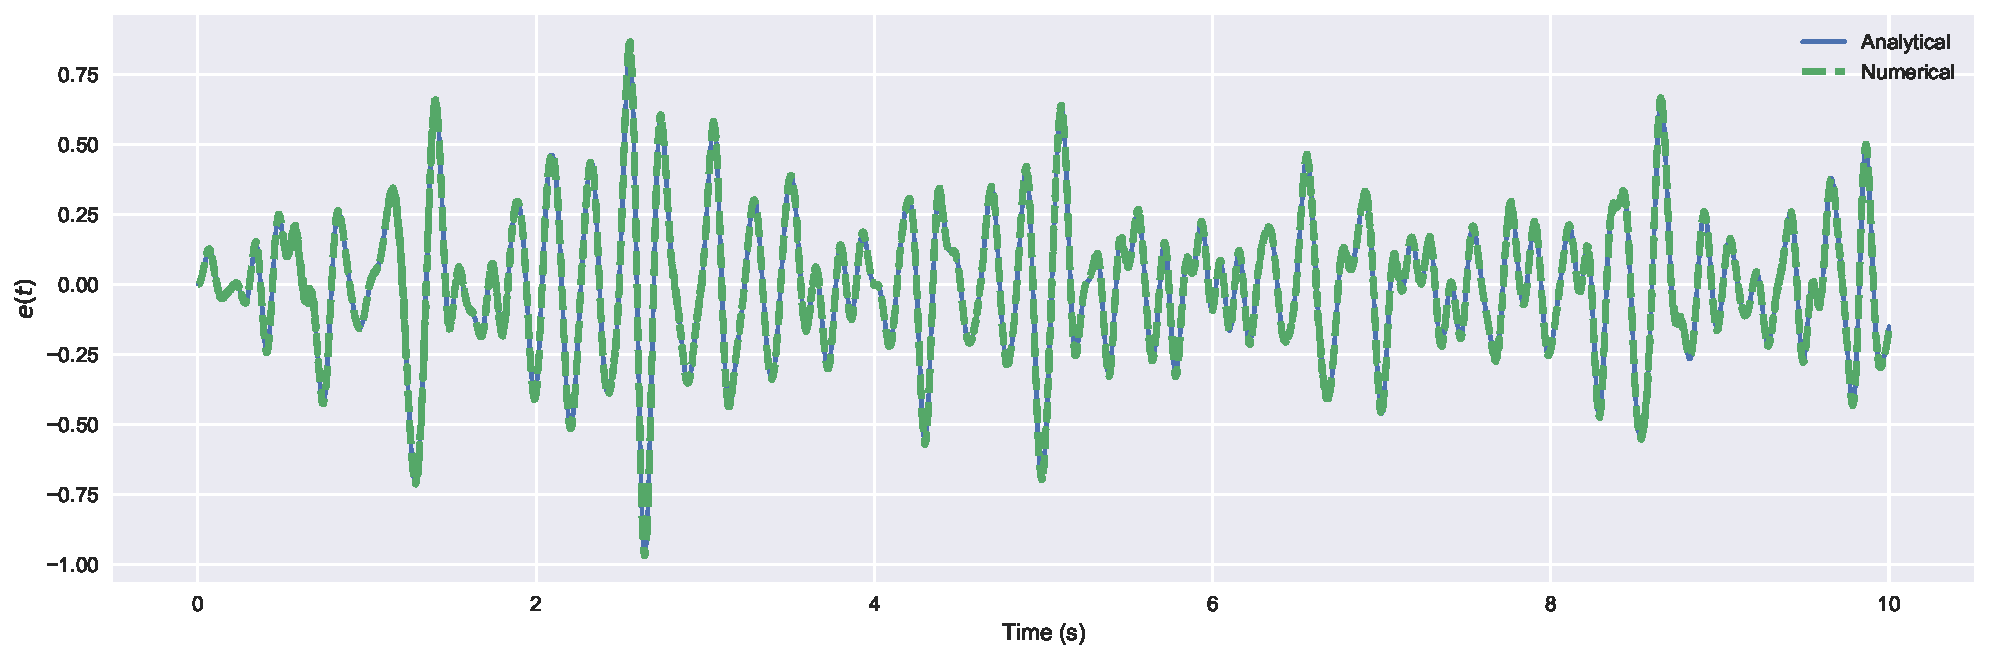
\includegraphics[width=1.0\textwidth]{pes-error}
\caption{ \label{fig:pes-error}
  Comparison of the analytical error (equation~\ref{eq:lowpass-solution}) to the numerical $e(t)$ obtained by simulating the network from Figure~\ref{fig:pes-filtered-network} ($\kappa = \numprint{e-3}$).
  The control signal $r(t)$ is randomly sampled white noise with a cutoff frequency of $10\,$Hz.
  The normalized root-mean-square error is approximately $3.7\%$.
}
\end{figure}

\begin{figure}
\centering
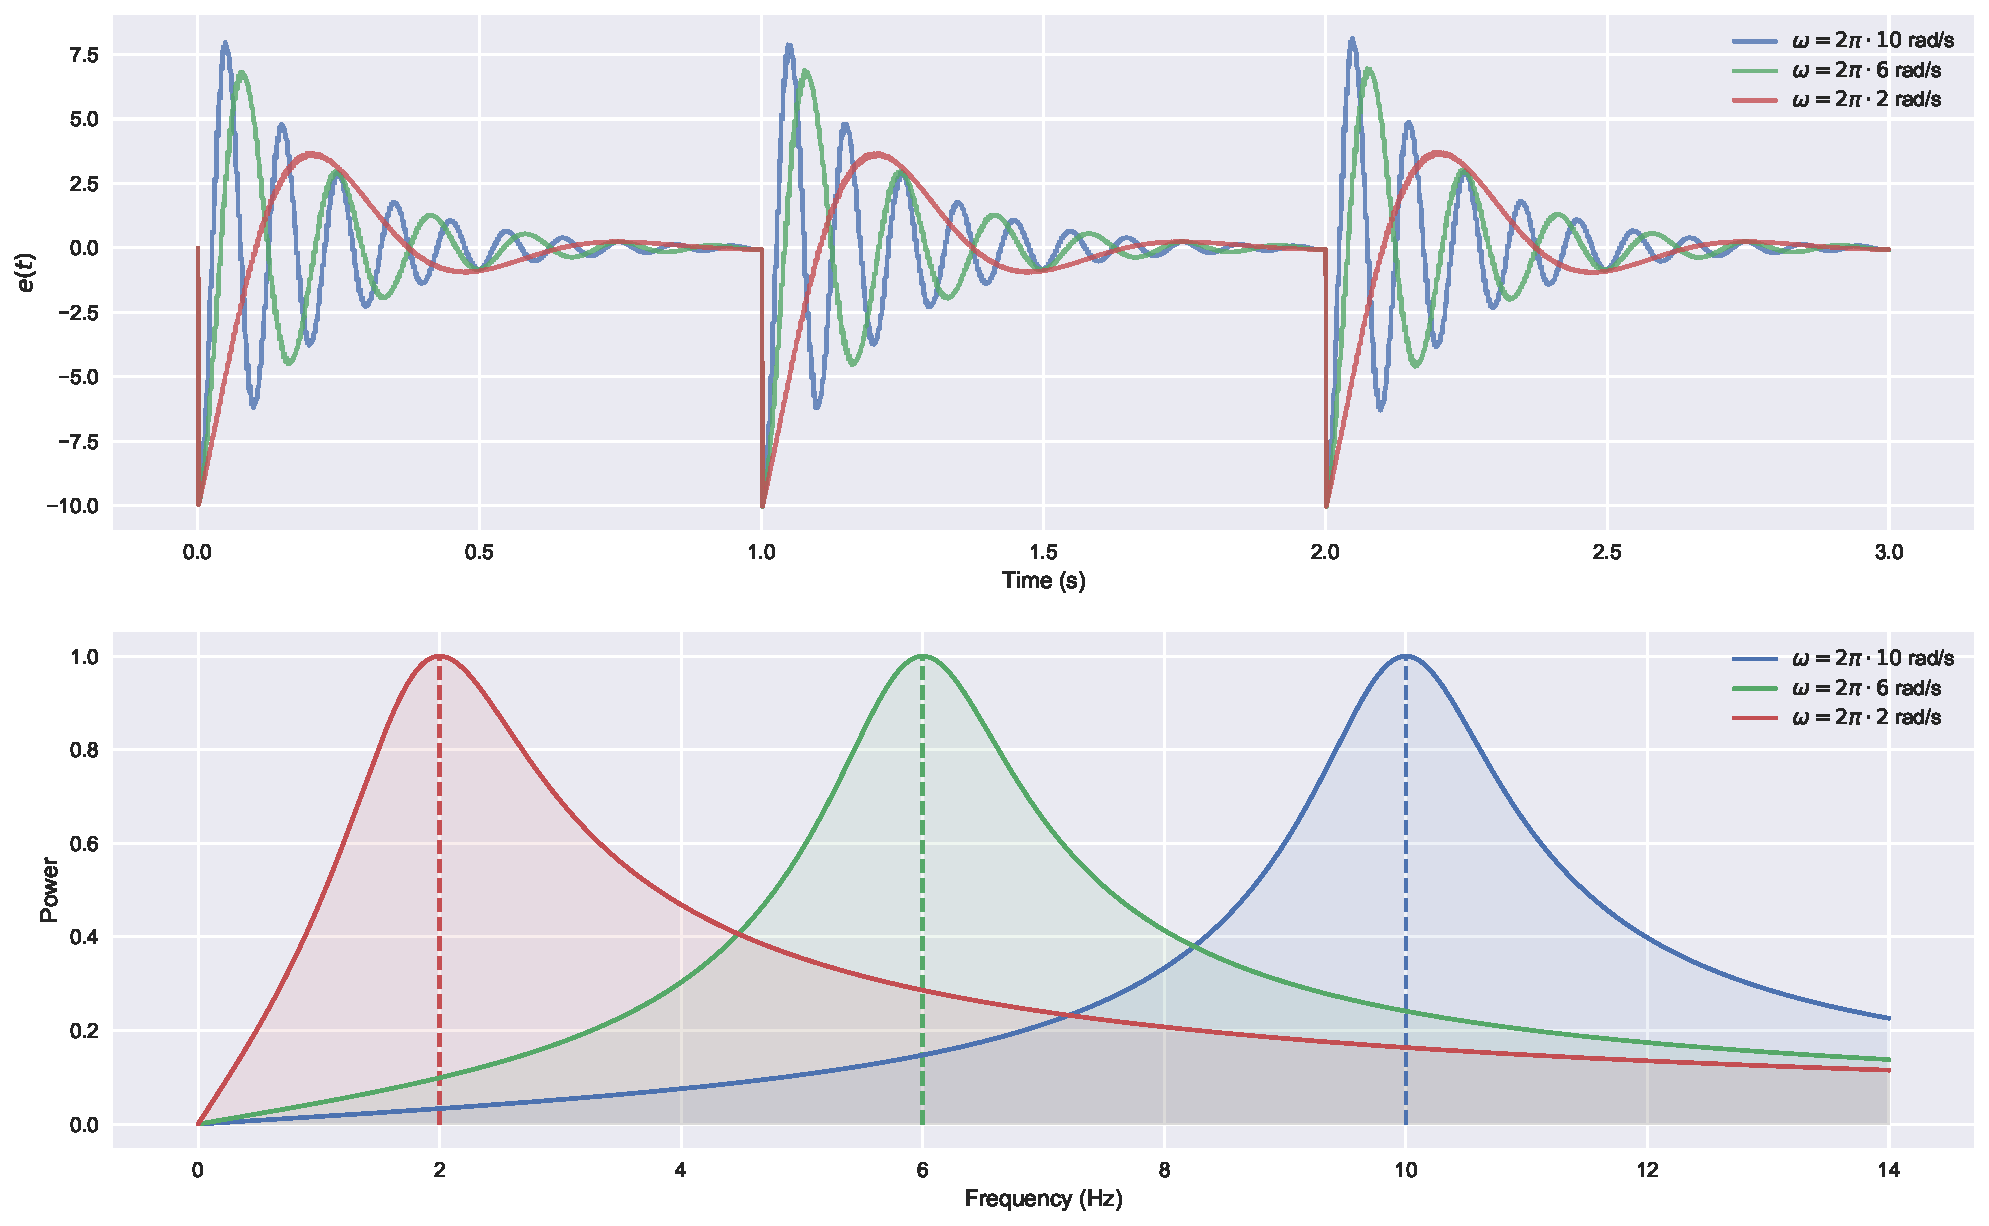
\includegraphics[width=1.0\textwidth]{pes-oscillator}
\caption{ \label{fig:pes-oscillator}
  Harnessing the dynamics of PES with various $\kappa$ to engineer decaying oscillators with predetermined frequencies ($\omega$) and bandwidths ($Q$).
  The time constant of the first-order lowpass filter is fixed at $\tau = 0.1\,$s, while $\kappa$ is set to achieve the desired $\omega$ via equation~\ref{eq:bandpass-w}.
  (Top)~Once every second, $r(t)$ is set to a unit-area impulse.
  Consequently, $e(t)$ oscillates according to the impulse response, $f(t)$.
  (Bottom)~Visualizing the ideal frequency response of $F(s)$ (equation~\ref{eq:lowpass-solution}).
  Dashed lines at $\omega$ (equation~\ref{eq:bandpass-w}) align with the peak of each bandpass filter, or equivalently the frequency of each oscillation.
  The width of each filter is proportional to the decay rate $Q^{-1}$ (equation~\ref{eq:bandpass-Q}).
}
\end{figure}

\subsubsection{Discussion}

Since $\phi = \tau \kappa \|\V{a}\|^2 > \frac{1}{4}$ if and only if the weights oscillate, this motivates a simple heuristic for setting the learning rate to prevent oscillatory weight changes: set $\kappa \le \frac{1}{4 \tau \|\V{a}\|^2}$, where $\|\V{a}\|^2$ is maximal over all possible activity vectors.
In this case, equation~\ref{eq:lowpass-solution} factors into a (differentiated) double-exponential:
\begin{equation*}
F(s) = \frac{-\tau_1 \tau_2 s}{\tau (\tau_1 s + 1)(\tau_2 s + 1)} = \left( - \tau_1 \tau_2 \tau^{-1} s \right) \left( \frac{1}{\tau_1 s + 1}\right) \left(\frac{1}{\tau_2 s + 1}\right) \text{,}
\end{equation*}
that is, two first-order lowpass filters chained together, where:
\begin{equation*}
\left( \tau_1, \tau_2 \right) = \frac{2 \tau}{1 \mp \sqrt{1 - 4 \phi}} \text{,}
\end{equation*}
by equation~\ref{eq:poles}.
In other words, the non-oscillatory regime ($0 < \phi \le \frac{1}{4}$) of PES is characterized by the dynamics of a double-exponential.
We remark that $\tau_1 = \tau_2 = 2 \tau$ (i.e.,~an alpha filter) directly on the point of bifurcation from double-exponential to oscillatory behaviour ($\phi = \frac{1}{4}$; see Figure~\ref{fig:pes-poles}).

In all applications involving online learning (that we are aware of) oscillatory weight changes are viewed as problematic, and so the relevant constants ($\tau$, $\kappa$, and $\| \V{a} \|^2$) are tweaked until the issue disappears.
In contrast, we have shown that not only can the relationship between these constants and the oscillations be fully understood, but they can be harnessed to engineer bandpass filters (with respect to the transformation $r(t) \mapsto e(t)$) with specific frequencies ($\omega$) and bandwidths ($Q$).
More generally, the PES learning rule can be used to construct dynamical systems whose transfer function (equation~\ref{eq:s-domain}) depends on $H(s)$, $\kappa$, and $\| \V{a} \|^2$.
As we used only a single spiking neuron, the accuracy of these systems rely solely on the accuracy of the PES implementation, the model of $H(s)$, and the constancy of $(\V{a} \ast h)(t)$ in practice (i.e.,~given spiking activity).

Although we have analyzed the continuous-time setting, the same proof technique can be applied to the discrete-time domain by use of the $Z$-transform.
Likewise, although we have assumed $x$ is a constant, we can apply a ``separation of timescales'' argument (i.e.,~assuming $x(t)$ changes on a slower timescale than $f(t)$) to carry this same analysis over to dynamic $x(t)$.
%More precisely, bounding the real components of equation~\ref{eq:poles} above by $c$,
%\footnote{Strictly, $c = -\frac{1}{2\tau}$ for the oscillatory case, and $c = \frac{-1 + \sqrt{1 - 4 \tau \kappa \|\V{a}\|^2}}{2 \tau}$ otherwise.}
By equation~\ref{eq:poles}, this analysis holds approximately for $x(t)$ with frequencies $\ll -\frac{1}{4 \pi \tau}\,$Hz, by applying a time-varying filter to $\V{d}(t)$ that depends on the current activity vector.

In conclusion, we have extended our previous analysis of PES to include linearly filtered feedback and a dynamic reference signal.
This fully characterizes the rule in the context of NEF networks representing a constant value, as a transfer function from the reference signal to the error signal.
This transfer function may then be readily analyzed and exploited using linear systems theory.
This demonstrates a more general principle of recurrently coupling available dynamical primitives in biological models (here, a PSC that is integrated by an online learning rule) to improve network-level computations.
% If we can find ways to exploit these things, then nature almost certainly can...

\begin{figure}
\centering
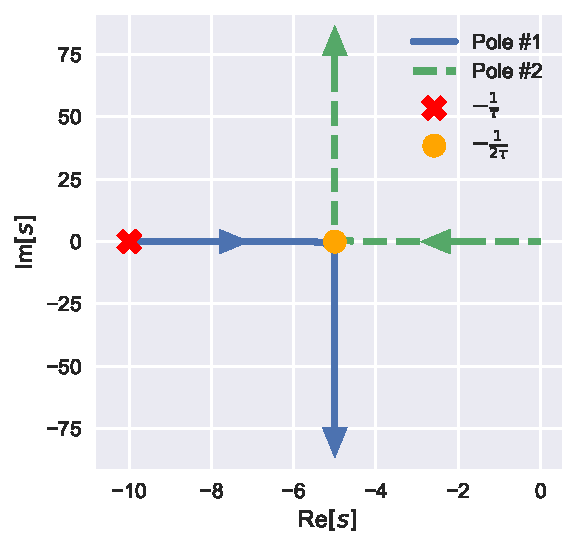
\includegraphics[width=0.6\textwidth]{pes-poles}
\caption{ \label{fig:pes-poles}
  Visualizing the poles of $F(s)$ (equation~\ref{eq:poles}) by sweeping $\kappa > 0$ (while $\| \V{a} \|^2$  and $\tau = 0.1\,$s remain fixed).
  Arrows follow the direction of \emph{increasing} $\kappa$.
  When $\phi \le \frac{1}{4}$, the dynamics of PES are a double-exponential.
  The learning rule becomes an alpha filter when the two poles collide: $\phi = \frac{1}{4} \iff s = -\frac{1}{2\tau}$ (marked by a solid circle).
  When $\phi > \frac{1}{4}$, the weight changes become oscillatory (due to complex poles).
  As $\kappa$ increases, the oscillatory frequency, $\omega$, scales as $\mathcal{O}\left(\sqrt{\kappa}\right)$.
  As $\kappa$ decreases, the first pole converges to $s = -\frac{1}{\tau}$ (marked by a solid \texttt{x}) while the second pole cancels the zero at $s = 0$. %(i.e.,~$F(s) = -H(s)$, $s \ne 0$).
}
\end{figure}

\subsection{Dynamics of Saturation}

Characterizing saturation as a dynamical system

\subsection{Dynamics of Error}

Writing down the dynamical system arising from the error term. e.g., oscillator error.

